\documentclass[]{foi} % zakomentirati za pisanje rada na engleskom jeziku
% \documentclass[english]{foi} % odkomentirati za pisanje rada na engleskom jeziku
\usepackage[utf8]{inputenc}
\usepackage{lipsum}

\vrstaRada{\projekt}
% \zavrsni ili \diplomski ili \seminar ili \projekt

\title{Implementacija Web poslužitelja korištenjem funkcijskog pristupa}
\predmet{\predmetDP}
% ostaviti prazno ako \vrstaRada nije \projekt ili \seminar
% \predmetBP ili \predmetDP ili \predmetTBP ili \predmetVAS

\author{Hrvoje Lesar} % ime i prezime studenta/studentice
\spolStudenta{\musko} % \zensko ili \musko

\mentor{Bogdan Okreša Đurić} % ime i prezime mentora
\spolMentora{\musko} % \zensko ili \musko
\titulaProfesora{dr. sc.}
% HR: dr. sc.  / doc. dr. sc. / izv. prof. dr. sc. / prof. dr. sc. 
% EN: -prazno- / Asst. Prof.  / Assoc. Prof.       / Full Prof.

\godina{2023}
\mjesec{Siječanj} % mjesec obrane rada ili projekta

\indeks{0016133479} % broj indeksa ili JMBAG

\smjer{Organizacija poslovnih sustava}
% (ili:
%     Informacijski sustavi, 
%     Poslovni sustavi, 
%     Ekonomika poduzetništva, 
%     Primjena informacijske tehnologije u poslovanju, 
%     Informacijsko i programsko inženjerstvo, 
%     Baze podataka i baze znanja, 
%     Organizacija poslovnih sustava, 
%     Informatika u obrazovanju
% )


\sazetak{Opsega od 100 do 300 riječi. Sažetak upućuje na temu rada, ukratko se iznosi čime se rad bavi, teorijsko-metodološka polazišta, glavne teze i smjer rada te zaključci.}

\kljucneRijeci{riječ; riječ; ...riječ; Obuhvaća $7\pm2$ ključna pojma koji su glavni predmet rasprave u radu.}

\begin{document}

\maketitle

\tableofcontents

\makeatletter \def\@dotsep{4.5} \makeatother
\pagestyle{plain}

\chapter{Uvod}

\chapter{Funkcijsko programiranje}

Funkcijsko programiranje je pristup programiranju koji se temelji na pozivima funkcija kao primarnom konstruktu programiranja.
Općenito pruža praktične pristupe rješavanju problema i pruža uvide u mnoge aspekte računarstva \cite{michaelson2011introduction}.
Posebno, sa svojim korijenima u teoriji računarstva, čini poveznicu između formalnih metoda u računarstvu i njihovu primjenu.

Funkcijsko programiranje kao osnovu koristi $\lambda$-račun što znači da se problemi rješavaju korištenjem
isključivo korištenjem funkcija i njihovih povratnih vrijednosti. Glavna svojstva koja imaju funkcijski
programski jezici su nepromjenjivost stanja varijabli, čistoća funkcija, funkcije višeg reda. Više o glavnim svojstvima
u poglavlju \ref{sec:svojstva}. U funkcijskom programiranju programski kod se sastoji od definicije jedne
ili više funkcija, a izvođenje programa svodi se na izračunavanje funkcijskih izraza \cite{rovzic2016lambda}.

\section{Glavna svojstva funkcijskih programskih jezika} \label{sec:svojstva}

Funkcijsko programiranje nije ograničeno samo na funkcijske programske jezike,
mnogi multiparadigmatski jezici omogućavaju funkcijski stil programiranja, no kod takvih je
potrebno poštivati sljedeća svojstva \cite{rovzic2016lambda}:
\begin{itemize}
	\item Nepromjenjivost stanja varijabli; Vrijednost varijable, objekta nije moguće promijeniti
	      nakon inicijalizacije. Ovakav pristup stvara veću sigurnost kod korištenja varijabli jer
	      smo sigurni da se varijabla kroz cijeli tok programa neće promijeniti. Kako bi se kreirale
	      nove varijable potrebno je izvršavanje funkcija koje vraćaju neku vrijednost.
	\item Čiste funkcije; Funkcije koje ne ovise o nikakvim vanjskim varijablama. Koriste jedino vrijednosti
	      koje su proslijeđene direktno u funkciju, te vrijednost prema svojstvu nepromjenjivosti ne može mijenjati.
	      Čiste funkcije garantiraju vraćanje iste vrijednosti prosljeđivanjem istih vrijednostu u funkciju,
	      ovo svojstvo pomaže kod optimizacije jer je funkciju potrebno pokrenuti i izračunati jedanput.
	      Čiste funkcije nemaju popratne posljedice osim kalkulacije razultata. Takav pristup eliminira
	      veliki izvor greška u programu i čini redoslijed izvršavanja nebitnim jer ne postoje popratne
	      posljedice te funkcija može biti evaluirana u bilo kojem trenutku \cite{hughes1989functional}.
	\item Funkcije prvog i višeg reda; Funkcije su tretirane kao objekti prvog reda tj. mogu biti rekurzivne,
	      višeg reda, polimorfne \cite{10.1145/72551.72554}. Funkcije višeg reda mogu primati kao argumente
	      druge funkcije te mogu vraćati funkcije kao povratne vrijednosti.
\end{itemize}

\chapter{Web poslužitelj}

Web poslužitelj u svojem najosnovnijem obliku isporučuje klijentima zatražene dokumente preko weba.
Web se sastoji od tri glavne komponente \cite{yeager1996web}:
\begin{enumerate}
	\item Sistem adresa, URL-a (engl. Universal Resource Locators); Putanje koje omogućuju korisnicima
	      dohvaćanje gotovo bilo koju vrstu informacija s gotovo bilo kojeg mjesta na internetu
	\item HTTP (engl. HyperText Transfer Protocol); Najčešće korišteni protokol za komunikaciju između
	      klijenta i poslužitelja putem weba. Zbog svoje relativne jednostavnosti omogućuje mnogim programima
	      zajednički rad.
	\item HTML (engl. HyperText Markup Language); Najčešće posluživana vrsta dokumenta na webu te je može
	      koristiti svaki web preglednik.
\end{enumerate}

Web poslužitelj s klijentima komunicira razmjenom poruka. Uspostavom veze između poslužitelja i klijenta,
klijent može poslati zahtjev poslužitelju. U slučaju HTTP-a klijent šalje zahtjev s određenom metodom,
ovisno o metodi šalje samo zaglavlje ili zaglavlje i tijelo poruke. HTTP zaglavlja su u tekstualnom obliku.
Poslužitelj, kod primanja zaglavlja, interpretira zahtjev klijenta i pokušava ga ispuniti. Ovisno o
uspjehu ispunjenja zahtjeva poslužitelj šalje povratnu informaciju klijentu, povratna informacija se sastoji
od HTTP zaglavlja i ovisno o zahtjevu, neke HTML datoteke, teksta, slike, strukturiranih podataka.

\section{Primjer HTTP zahtjeva i odgovora}

Sljedeće predstavlja jednostavni HTTP zahtjev poslan s klijenta na poslužitelj:
\begin{verbatim}
GET /index.html HTTP/1.1
Accept: text/html,application/xml,image/webp,image/apng,*/*
User-Agent: Mozilla/5.0  Gecko/20100101 Firefox/108.0
\end{verbatim}

HTTP zahtjev počinje u prvoj liniji s metodom koju slijedi URL putanja te HTTP verzija, u ovom slučaju verzija 1.1.
Druga linija ukazuje kakve vrste dokumenata i podataka je klijent spreman primiti. U primjeru klijent eksplicitno ukazuje da
može primiti html, xml, webp ili bilo koju drugu vrstu datoteke na što ukazuje */* dio.
Zadnja linija identificira tip preglednika s kojega je poslan zahtjev.

Poslužitelj za zahtjev kreira odgovor. Odgovor uvijek u prvoj liniji sadrži status odgovora tj.
je li zahtjev uspio ili je odbijen. Sljedeće sadrži informacije o odgovoru, to su slično kao
kod zahtjeva, informacije o stvarnim zahtijevanim podacima, informacije o poslužitelju,
vrstu podataka koji se šalju. Zadnji dio odgovora je dokument ili podatci koje je klijent
zatražio. Sljedeće je primjer odgovora na prije postavljeni zahtjev:
\begin{verbatim}
HTTP/1.1 200 OK
Content-Type: text/html
Content-Lenght: 40

<html>
<h1>Hello World!</h1>
</html>
\end{verbatim}
Prva linija odgovora je status odgovora, odgovor na zahtjev je uspješan što se može vidjeti iz
numeričke reprezentacije statusa 200 ili iz OK. Druga linija opisuje tip dokumenta koji je poslan
u odgovoru. U ovom slučaju je to html dokument, duljine 40 bajta. Prazna linija je odjeljak
zaglavlja odgovora i tijela odgovora. Ispod prazne linije nalazi se tijelo odgovora. Tijelo može
biti u tekstualnom ili binarnom obliku i u odgovorima sa tijelom se uvijek nalazi iza odjeljka.

\chapter{Implementacija web poslužitelja}

\section{Odabrani programski jezik i upute za pokretanje} \label{sec:pokretanje}
Web poslužitelj je implementiran u typescriptu, zbog lakšeg definiranje tipova podataka
i razumijevanja koda. Typescript je sintaktički nadskup javascript-a i potrebno ga je
konvertirati u javascript tj. transpilirati.

Za kompajliranje i pokretanje web poslužitelja potrebni su NodeJS, npm (node package manager) i typescript.
Ako su NodeJS i npm instalirani typescript se može globalno instalirati pokretanjem \texttt{npm install -g typescript}
u terminalu. Za pokretanje projekta potrebno se je postaviti u direktorij s datotekama \texttt{package.json} i
\texttt{tsconfig.json}. U tom direktoriju prvo pokrenuti \texttt{npm install} da npm pribavi potrebne pakete
za pokretanje programa (Program jedino zavisi o paketu \texttt{@types/node} koji sadrži NodeJS tipove za typescript).
Nakon pribavljanja paketa potrebno je transpilirati program što se odrađuje pokretanjem \texttt{tsc}, završetkom
transpilacije web poslužitelj se može pokrenuti s \texttt{node src/main.js}. Web poslužitelj se pokreće na
adresi \texttt{0.0.0.0:8888} ili \texttt{localhost:8888}.

Za potrebe lakšeg pokretanja u projektu je postavljena već transpajlirana javascript datoteka 
web poslužitelja, pošto je ta datoteka generirana od strane transpajlera ne 
mora biti pogodna za čitanje izvornog koda. Za čitanje izvornog koda predlaže se
\texttt{main.ts} datoteka. Svi sljedeći isječci koda će sadržavati typescript.

\section{Implementacija}

Poslužitelj je implementiran poštivanjem funkcijskog pristupa, no neke funkcije nisu
potpuno "čiste" pošto moraju pisati na mrežu ili čitati sa diska. Sljedeća funkcija
pokreće web poslužitelj:
\begin{lstlisting}[caption={Funkcija za pokretanje web poslužitelja}, label=lst:pokretanje]
const createServer = (hostname: string, port: number, ...routes: Route[]) => {
    new net.Server()
        .listen(port, hostname, undefined, () => {
            console.log(`Server started on ${hostname}:${port}.`);
        })
        .on("connection", (socket: net.Socket) => {
            handleNewConnection(socket, routes);
        });
};
\end{lstlisting}
Funkcija kao ulaz prima hostname i port na kojemu se kreira server te varijabilni broj
ruta tj. putanja na kojima će pokušati odgovoriti na zahtjev klijenta. Metoda listen()
registrira server na unesenim hostname-u i portu, a metoda on() registrira događaj (event)
connection što poziva funkciju kad događaj okine.

Kod kreiranja poslužitelja potrebno je definirati na koje putanje će pokušati nešto izvršiti
te dati prikladan odgovor na zahtjev. Za sve putanje koje nisu definirane poslužitelj odgovara
sa 404 NOT FOUND. Ruta je definirana metodom koju očekuje (GET, POST), putanjom koju očekuje
i funkcijom koja će se izvršiti kod odgovaranja na zahtjev.
\begin{lstlisting}[caption={Definicija rute}, label=lst:ruta]
const route = (
    method: string,
    path: string,
    action: (socket: net.Socket, request: Request | undefined) => void
): Route => {
    return {
        method,
        path,
        action,
    };
};
\end{lstlisting}

Ovu funkciju poziva poslužitelj kod prihvaćanja nove veze i primanja zahtjeva od
klijenta. Funkcija nije čista jer koristi try, catch mehanizam, no u ovom slučaju
je potrebno jer inače kod greške na socketu bi se poslužitelj srušio. Funkcija nakon
primanja HTTP zahtjeva parsira zahtjev u strukturu pogodnu za program. Nakon toga pokuša
odrediti ako ruta odgovara nekoj od zadanih i ako pripada poziva funkciju koja generira
odgovarajući odgovor na zahtjev.
\begin{lstlisting}[caption={Prihvaćanje nove veze i zahtjeva}, label=lst:conn]
const handleNewConnection = (socket: net.Socket, routes: Route[]) => {
    socket.on("data", (buffer) => {
        try {
            const request = parseRequest(buffer.toString("utf8"));
            if (request) {
                const route = matchRoute(request, routes);
                if (route) {
                    const [nRequest, nRoute] = route;
                    nRoute.action(socket, nRequest);
                } else {
                    writeNotFoundToSocket(socket);
                }
            } else {
                writeNotFoundToSocket(socket);
            }
            socket.pipe(socket).end();
        } catch (e) {
            console.error(e);
        }
    });
};
\end{lstlisting}

\subsection{Rute} \
Web poslužitelj podržava tri vrste ruta.
\begin{enumerate}
	\item Puno definirane rute (/path/to/index.html);
	\item Wildcard rute (/path/to/*). Kod ove vrste ruta sve putanje nakon znaka \texttt{*}
	      su validne i poslužitelj će ih pokušati poslužiti
	\item Rute s varijabilnom putanjom (/path/\{to\}/\{resource\}). Ovakav tip ruta je koristan
	      pošto se vrijednosti u zagradama \texttt{varijabla} tretiraju kao varijable.
	      Primjer može biti pregled određenog zapisa u bazi podataka prema nekom identifikatoru
	      (GET /user/\{id\}).
\end{enumerate}
Web poslužitelj također ima mogućnost čitanja (samo na zadnjem dijelu putanje) niz upita (query
string). Niz upita nije posebno definiran kod kreiranja rute, već svaka ruta parsira
niz upita, ako postoji, te ga je moguće koristiti po potrebi.

Ova funkcija se prosljeđuje kao argument u \texttt{createServer} funkciju kako bi se
registrirala nova ruta na poslužitelju. Poslužitelj će na GET metodu koja ima putanju
\texttt{/} ili praznu putanju generirati odgovor čitanjem datoteke \texttt{index.html},
kreirati će odgovarajuće zaglavlje i u tijelo HTTP odgovora će dodati sadržaj pročitane
datoteke. Sljedeći isječak koda je primjer definiranje rute, sve rute su definirane u
poglavlju \ref{sec:rute}.
\begin{lstlisting}[caption={Primjer rute}, label=lst:primjer_rute]
route(HTTPMethods.GET, "/", (socket) => {
    compose(
        ([file, socket]: [string, net.Socket]) => {
            compose(
                ([response, socket]: [string, net.Socket]) => {
                    socket.write(response);
                },
                ([file, socket]: [string, net.Socket]) => {
                    return [
                        makeResponse(
                            STATUSCODES.OK,
                            [
                                ["Content-Lenght", file.length.toString()],
                                ["Content-Type", "text/html"],
                            ],
                            file
                        ),
                        socket,
                    ];
                }
            )([file, socket]);
        },
        (socket: net.Socket) => {
            return [
                readFileSync("./websites/index.html", {
                    encoding: "utf8",
                }),
                socket,
            ];
        }
    )(socket);
}),
\end{lstlisting}

Možemo primijetiti da kreirana ruta koristi funkciju \texttt{compose}. Compose radi
kompoziciju funkcija, funkcije se izvršavaju u obrnutom redoslijedu od napisanog,
zadnje definirana funkcija se prva izvršava te je rezultat izvršavanja funkcije
proslijeđen u sljedeću funkciju. U ovom slučaju kao ulazni argument \texttt{compose} funkcija
uzima \texttt{socket} koji je proslijeđen u anonimnu funkciju koja čita datoteku i vraća
sadržaj datoteke i socket, kako bi ih sljedeća funkcija mogla koristiti.

Funkcija \texttt{compose} je definirana na sljedeći način. Ulazni argument u funkciju je
varijabilni broj drugih funkcija. \texttt{Compose} vraća anonimnu funkciju koja kod poziva
prosljeđuje dani argument zadnjoj funkciji u kompoziciji i radi redukciju funkcija tj.
poziva svaku proslijeđenu funkciju u \texttt{compose} sa rezultatom prijašnje funkcije
u kompoziciji.
\begin{lstlisting}[caption={Definicija compose funkcije}, label=lst:compose_funkcija]
const compose = (...func: any[]) => {
    return (x: any) => {
        return func.reduceRight((prev, f) => f(prev), x);
    };
};
\end{lstlisting}


\subsection{Definirane rute} \label{sec:rute}

Lista ruta na koje će trenutna implementacija web servera dati odgovore.
Rute su zapisane u obliku \texttt{METODA} \texttt{/PUTANJA} - objašnjenje.
\begin{itemize}
	\item \texttt{GET} \texttt{/} - Poslužuje index.html dokument koji ima primjere
	      za ostale putanje.
	\item \texttt{GET} \texttt{/websites/*} - Poslužuje sve putanje koje počinju sa /websites
	\item \texttt{GET} \texttt{/demo/\{variable\}/path/\{uri\}} - Primjer varijabilne putanje.
	      Vraća JSON objekt koji kao ključeve ima variable i uri, a vrijednosti će odgovarati
	      vrijednostima koje će biti napisane na mjestu variable i uri u putanje. Odlazak na
	      putanju /demo/changeme/path/value će vratiti ovakav JSON objekt: \{"variable": "changeme", "uri": "value"\}.
	\item \texttt{GET} \texttt{/query} - Putanja za prikaz rada niza upita. Na kraj putanje može
	      se dodati upit tipa \texttt{?field=value\&anotherField=anotherValue}, te će poslužitelj
	      vratiti JSON objekt s unesenim upitom tj. upitima ako ih je više.
	\item \texttt{GET} \texttt{/form} - Učitava stranicu s primjerom slanja obrasca na poslužitelj.
	\item \texttt{POST} \texttt{/form} - Putanja za prihvaćanje poslanog obrasca.
    \item \texttt{GET} \texttt{/getData} - Dohvaća JSON objekt podataka prihvaćenih \texttt{POST /form} rutom.
\end{itemize}

\section{Prikaz rada aplikacije}

Način pokretanja web poslužitelja je opisan u poglavlju \ref{sec:pokretanje}. Kod pokretanja
poslužitelj registrira definirane rute i čeka na nove zahtjeve od klijenti. Jedino što
web poslužitelj ispisuje, nakon pokretanja, je hostname i port na kojemu je pokrenut te
eventualno ispisuje ako se je dogodila kakva greška, nema drugih ispisa.

Postavljeno je da se poslužitelj pokreće na adresi \texttt{0.0.0.0:8888}. Na adresu se
možemo povezati preko web pretraživača odlaskom na putanju \texttt{localhost:8888}.
Povezivanjem na \texttt{localhost:8888/} web poslužitelj odgovara sljedećim dokumentom:
\begin{figure}[h!]
    \centering
    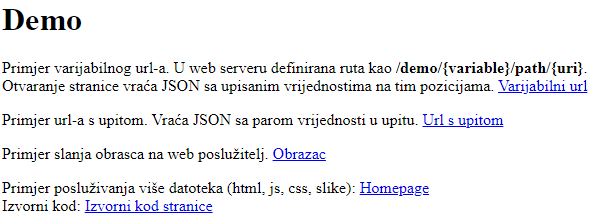
\includegraphics[width=0.9\textwidth]{slike/demo.png}
    \caption{Inicijalna stranica}
    \label{fig:init}
\end{figure}

Poslužena stranica sadrži primjere za svaku vrstu rute koju web poslužitelj podržava. Isto
tako koristi sve rute definirane u poglavlju \ref{sec:rute}. Prva putanja vodi na primjer
varijabilne putanje. Klikom na putanju web preglednik odlazi na putanju 
\texttt{/demo/changeme/path/value}. Poslužitelj će generirati i poslati JSON objekt
klijentu koji će biti prikazan ovisno o vrijednostima na pozicijama \texttt{changeme} i
\texttt{value}. Sljedeće je prikaz odgovora koji poslužitelj šalje klijentu za
zatraženu rutu \texttt{/demo/promijenjena/path/vrijednost}:

\begin{verbatim}
HTTP/1.1 200 Ok
Server:DP_PROJEKT
Content-Lenght:46
Content-Type:application/json

{"variable":"promijenjena","uri":"vrijednost"}
\end{verbatim}

Drugi primjer koji je postavljen na stranici je URL s upitom. Radi na sličan način kao
raniji primjer, ali umjesto definiranje duže rute na kraj rute se dodaje znak \texttt{?}
iza kojeg slijedi minimalno jedan upit. Upit se piše u obliku \texttt{polje=vrijednost}.
Moguće je postaviti više upita, za postavljanje više od jednog upita potrebno ih je odvojiti
znakom \texttt{\&}. Primjer URL-a s više upita 
\texttt{/query?polje=vrijednost\&drugoPolje=novaVrijednost\&upit=odgv}.
Sljedeće je prikaz odgovora koji poslužitelj generira za prethodni upit: 
\begin{verbatim}
HTTP/1.1 200 Ok
Server:DP_PROJEKT
Content-Lenght:66
Content-Type:application/json

{"polje":"vrijednost","drugoPolje":"novaVrijednost","upit":"odgv"}
\end{verbatim}

Treći primjer otvara stranicu s obrascem za ispunu. Stanica se sastoji od dva različita
polja za unos. Tipke za podnijeti obrazac i prikaza zapisa koji su bili poslani. Slika
prikazuje inicijalni izgled stranice prije nego postoji bilo koji zapis:
\begin{figure}[h!]
    \centering
    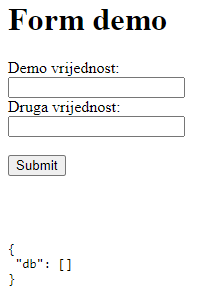
\includegraphics[width=0.2\textwidth]{slike/form.png}
    \caption{Prikaz stranice s obrascem}
    \label{fig:form}
\end{figure}

Ispunjavanjem forme i pritiskom na tipku \texttt{Submit} web preglednik na poslužitelj 
šalje sljedeće:
\begin{verbatim}
POST /form HTTP/1.1
Accept: */*
Accept-Encoding: gzip, deflate, br
Accept-Language: en-US,en;q=0.9
Connection: keep-alive
Content-Length: 15
Content-Type: application/x-www-form-urlencoded
Host: localhost:8888
Origin: http://localhost:8888
Referer: http://localhost:8888/form
Sec-Fetch-Dest: empty
Sec-Fetch-Mode: cors
Sec-Fetch-Site: same-origin
Sec-GPC: 1
User-Agent: Mozilla/5.0  Gecko/20100101 Firefox/108.0

demo=Demo&value2=v2
\end{verbatim}
Poslužitelj prema zadanom \texttt{Content-Type} zaglavlju parsira
primljene podatke. Dodaje ih u datoteku i generira odgovor koji se sastoji
od svih zapisa koji su u datoteci. Stranica će biti promijenjena kod sljedećih
učitavanja i imati će ovakav oblik:
\begin{figure}[h]
    \centering
    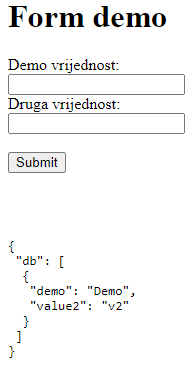
\includegraphics[width=0.2\textwidth]{slike/form2.png}
    \caption{Stranica s obrascom i jednim zapisom}
    \label{fig:form2}
\end{figure}

Donji dio stranice će prikazivati sve zapise koji su spremljeni na poslužitelji
i rasti će dodavanjem novih zapisa.

Posljednji primjer učitava web stranicu koja će zatražiti još dokumenti. Za očekivan
prikaz stranice, stranica treba učitati jednu \texttt{.js} datoteku, jednu \texttt{.css}
datoteku i tri \texttt{.png} datoteke. Kako na poslužitelju nebi bilo potrebno za svaku
datoteku postavljati posebnu rutu za posluživanje samo jedne datoteke, poslužitelj
koristi definiranu wildcard rutu \texttt{/websites/*}. Zbog te rute poslužitelj može
pribaviti sve potrebne datoteke za prikaz stranice sa svim slikama i stilom.
Za sve datoteke koje pribavlja će prema ekstenziji pokušati postaviti odgovarajuće
\texttt{Content-Type} zaglavlje, no ako ekstenzija nije specificirana u zaglavlje piše
\texttt{text/plain}, što u nekim slučajevima može dovesti do problema kod učitavanja
stranica, pošto preglednik može odbiti datoteku koju prepoznaje, ali ima zapisano krivo
\texttt{Content-Type} zaglavlje.
Slika prikazuje stanje mreže i sve zahtjeve poslane s klijenta na poslužitelj za
prikaz stranice:
\begin{figure}[h]
    \centering
    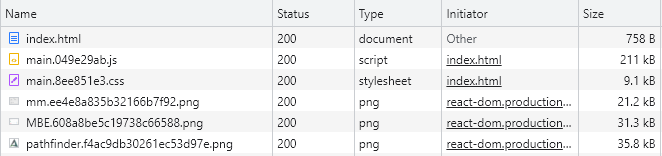
\includegraphics[width=\textwidth]{slike/mreza.png}
    \caption{Prikaz zahtjeva poslanih s klijenta}
    \label{fig:mreza}
\end{figure}


\chapter{Zaključak}

\lipsum[1-2]

\makebackmatter
% generira popis korištene literature, popis slika (ako je primjenjivo), popis tablica (ako je primjenjivo) i popis isječaka koda (ako je primjenjivo)
\end{document}
